\addtocontents{toc}{\protect\phasecrisp{Phase 2 --- Compréhension des données}}
\chapter{Exploration et compréhension des données}

\section*{Introduction}
\addcontentsline{toc}{section}{Introduction}

Le chapitre précédent a posé le problème et fixé les exigences. Celui-ci ouvre la deuxième phase de
la démarche, la compréhension des données. Un modèle ne vaut que ce que valent les données dont il
apprend, et l'exploration conduite ici décide de ce qui sera possible ensuite.

Nous décrivons d'abord la provenance du corpus, son schéma et la variable à prédire. Nous mesurons
ensuite sa qualité, sa distribution et sa redondance. L'analyse met au jour deux caractéristiques
qui pèsent sur toute la suite : une distribution très inégale entre catégories et une forte
redondance des situations décrites.

Aucune transformation n'est appliquée dans ce chapitre. Il observe, il mesure, et il énonce les
risques que ces mesures font peser sur la modélisation.

\section{Présentation des données}

Le corpus provient d'un export unique, dont nous décrivons la provenance, le schéma et la variable
à prédire avant toute analyse.

\subsection{Provenance et mode de collecte}

\label{sec:provenance}

Le jeu de données nous a été fourni par l'entreprise. Il rassemble les demandes traitées par le
service support dans le cadre de son activité courante : 1\,800 tickets créés entre le
1\textsuperscript{er} janvier 2025 et le 17 février 2026, soit quatorze mois d'activité et une
moyenne de 129 tickets par mois. Ils émanent de 202 demandeurs distincts répartis sur les huit
filiales du groupe, et sont assignés à onze intervenants, ce qui recoupe l'effectif du service
décrit au chapitre~1.

La saisie n'était soumise à aucun contrôle, ce dont le chapitre~1 donne l'illustration la plus
nette avec les deux formats de date qui coexistent dans un même champ. Les nettoyages que cet état
impose relèvent du chapitre~3 ; l'analyse qui suit porte sur le fichier tel qu'il a été reçu.

\subsection{Schéma et variable cible}

\label{sec:schema}

Chaque ticket est décrit par dix-huit champs. Le tableau~\ref{tab:schema} les regroupe par rôle
plutôt que dans l'ordre du fichier.

\begin{table}[!htbp]
\centering
\styletableau
\caption{Organisation des dix-huit champs du jeu de données}
\label{tab:schema}
\begin{tabular}{|Bp{2.6cm}|Lp{5.2cm}|Lp{5.8cm}|}
\hline
\rowcolor{enteteTab}
\textbf{Groupe} & \textbf{Champs} & \textbf{Rôle dans le projet} \\
\hline
Identification & \texttt{ID}, \texttt{CID} & Clé du ticket et référence de configuration \\
\hline
Contenu & \texttt{Titre}, \texttt{Description} & Entrée textuelle des modèles \\
\hline
Classement & \texttt{Catégorie}, \texttt{Classification}, \texttt{Priorité} & \texttt{Catégorie}
est la variable cible ; les deux autres servent de contexte \\
\hline
Acteurs & \texttt{Demandeur}, \texttt{Filiale}, \texttt{Assigné~à} & Traçabilité de la demande et
de son traitement \\
\hline
Suivi & \texttt{STATUT}, \texttt{Date de création}, \texttt{Date de résolution} & Traçabilité des
états du ticket \\
\hline
Résolution & \texttt{Résolution/Motif}, \texttt{Analyse}, \texttt{knowledge Base} & Matière de la
base de connaissances interrogée par le moteur RAG \\
\hline
Provenance & \texttt{Type d'élément}, \texttt{Chemin~d'accès} & Champs techniques hérités de
l'outil de gestion, non exploités par les modèles \\
\hline
\end{tabular}
\end{table}

La variable cible est le champ \texttt{Catégorie}, qui prend huit modalités : \emph{Microsoft},
\emph{Réseau}, \emph{Applicatifs}, \emph{Infrastructure}, \emph{Système}, \emph{Communication},
\emph{Sécurité} et \emph{Backup}. C'est le référentiel employé par le service, introduit au
chapitre~1.

L'annotation est fiable : à chaque libellé de titre présent dans le corpus correspond une catégorie
et une seule, sans exception. Ce constat écarte le bruit d'étiquetage comme explication des
performances observées au chapitre~6.

\section{Analyse exploratoire des données}

L'exploration cherche ce qui, dans le corpus, décidera de ce qu'un modèle pourra apprendre. Quatre
angles la composent : la distribution des catégories, la matière textuelle disponible, les statuts
du ticket et la diversité réelle des situations décrites.

\subsection{Distribution des catégories}

\label{sec:distribution}

Le référentiel compte huit catégories, dont l'usage réel est loin d'être uniforme.

\begin{figure}[!htbp]
\centering
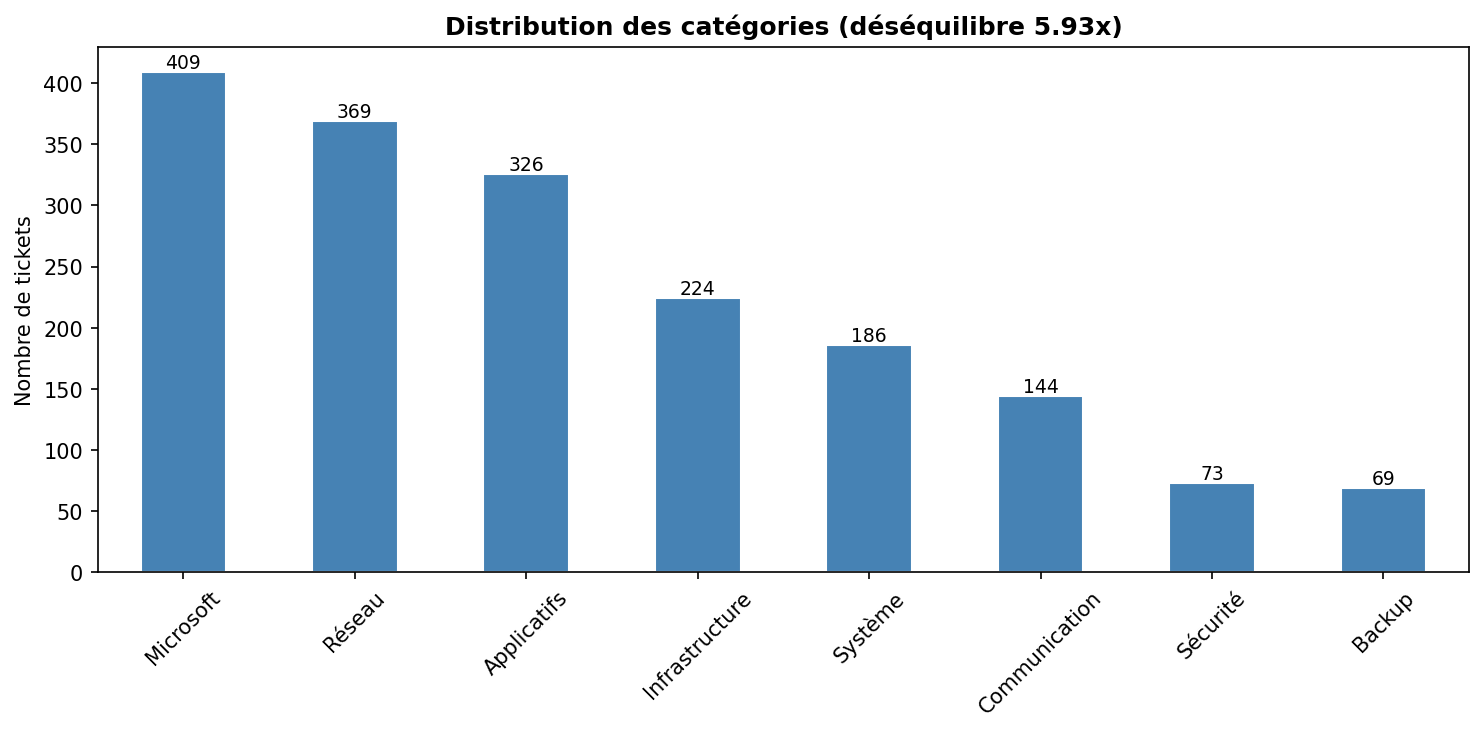
\includegraphics[width=0.94\textwidth]{ch03_distribution_categories.png}
\caption{Répartition des tickets par catégorie}
\label{fig:distcat}
\end{figure}

La distribution de la figure~\ref{fig:distcat} est nettement inégale. \emph{Microsoft} rassemble
409 tickets et \emph{Réseau} 369, quand \emph{Sécurité} en compte 73 et \emph{Backup} 69. Le rapport
entre la catégorie la plus fréquente et la plus rare atteint 5,93, et les trois premières
concentrent 1\,104 tickets, soit 61\,\% du corpus.

Ce déséquilibre est celui de l'activité réelle du service. Il pose une difficulté de modélisation :
un classifieur entraîné sans précaution privilégie les catégories abondantes, affichant une
exactitude globale élevée tout en échouant sur les catégories rares. Le problème est d'autant plus
gênant que \emph{Sécurité} est celle dont une erreur de classement coûte le plus cher.

\subsection{Complétude des champs et longueur des textes}

\label{sec:completude}

Douze des dix-huit champs sont renseignés sur la totalité des lignes, dont les quatre qui portent
l'information exploitée par les modèles : \texttt{Titre}, \texttt{Description}, \texttt{Catégorie}
et \texttt{knowledge Base}. La figure~\ref{fig:completude} donne le taux de remplissage des
dix-huit champs, le tableau~\ref{tab:completude} détaille les six incomplets.

\begin{figure}[!htbp]
\centering
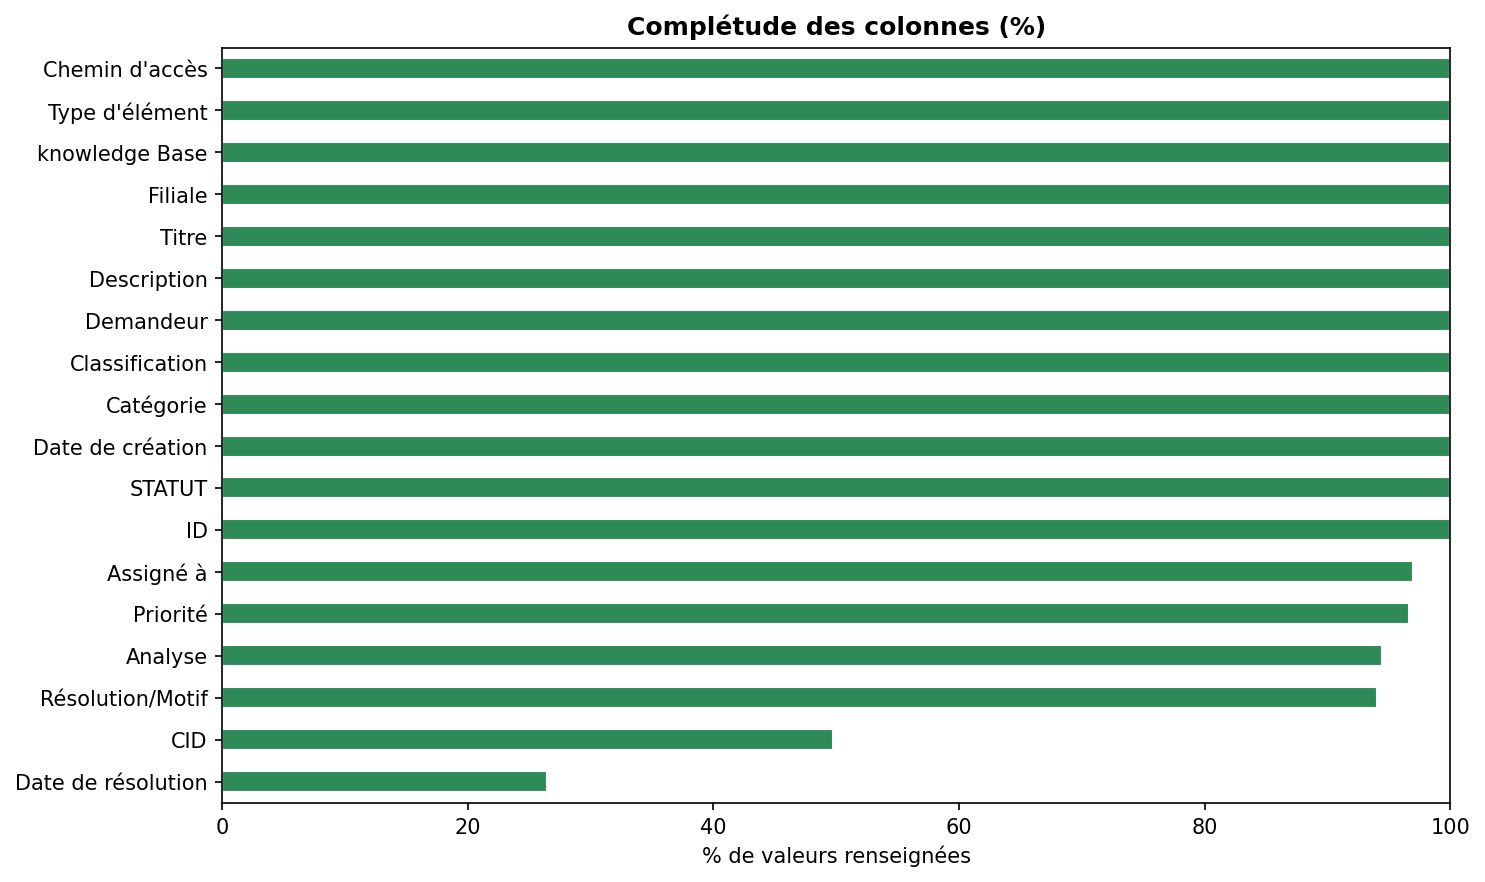
\includegraphics[width=0.92\textwidth]{ch03_completude.png}
\caption{Taux de remplissage des dix-huit champs du jeu de données}
\label{fig:completude}
\end{figure}

\begin{table}[!htbp]
\centering
\styletableau
\caption{Champs incomplets et interprétation}
\label{tab:completude}
\begin{tabular}{|Bp{3.4cm}|Cp{2.0cm}|Lp{7.4cm}|}
\hline
\rowcolor{enteteTab}
\textbf{Champ} & \textbf{Manquant} & \textbf{Interprétation} \\
\hline
\texttt{Date de résolution} & 73,6\,\% & Manquant par construction : seuls les 476 tickets au
statut \emph{Résolu} en portent une \\
\hline
\texttt{CID} & 50,3\,\% & Référence de configuration renseignée au cas par cas, sans caractère
obligatoire \\
\hline
\texttt{Résolution/Motif} & 5,9\,\% & Texte de clôture, qu'aucune règle de saisie n'impose \\
\hline
\texttt{Analyse} & 5,6\,\% & Champ de commentaire libre, facultatif \\
\hline
\texttt{Priorité} & 3,4\,\% & Non renseignée à la saisie \\
\hline
\texttt{Assigné à} & 3,1\,\% & Tickets non encore attribués au moment de l'export \\
\hline
\end{tabular}
\end{table}

Aucune de ces lacunes ne compromet le projet : les deux taux les plus élevés s'expliquent par la
nature des champs concernés, et les quatre autres restent sous 6\,\%. Le service renseigne
correctement les fiches qu'il traite ; ce qui manque relève du cycle de vie du ticket ou de champs
facultatifs.

Reste à savoir ce que contiennent les champs renseignés. Les descriptions sont courtes et
homogènes : de 23 à 46 mots, pour une médiane de 33, et les titres comptent de 2 à 8 mots. Aucun
ticket n'est vide ni aberrant par la longueur, comme le montre la distribution complète de la
figure~\ref{fig:longueurs}. Cette homogénéité dispense de tronquer ou de segmenter les textes avant
de les soumettre à un transformer.

% Placement [H] : la figure est large et basse, et une barriere de flottants lui
% laissait une page entiere. Ancree ici, elle suit le texte qui la commente et la
% sous-section suivante enchaine sur la meme page.
\begin{figure}[H]
\centering
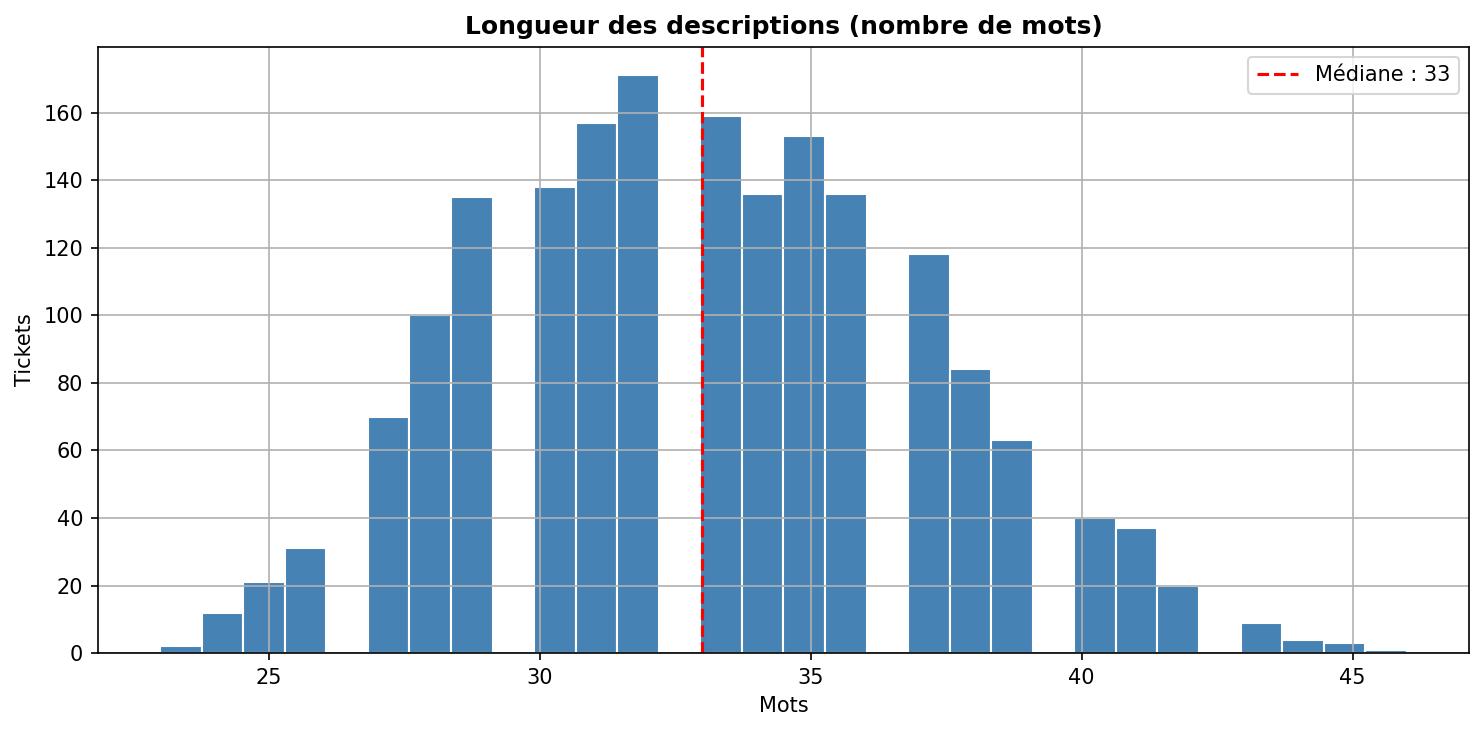
\includegraphics[width=0.86\textwidth]{ch03_longueurs.png}
\caption{Distribution de la longueur des descriptions, en nombre de mots}
\label{fig:longueurs}
\end{figure}

\subsection{Statuts, délais et décomptes du corpus}

\begin{table}[!htbp]
\centering
\styletableau
\caption{Répartition des tickets par statut}
\label{tab:statuts}
\begin{tabular}{|Bp{4.0cm}|Cp{2.4cm}|Cp{2.4cm}|}
\hline
\rowcolor{enteteTab}
\textbf{Statut} & \textbf{Tickets} & \textbf{Part} \\
\hline
Résolu & 476 & 26,4\,\% \\
\hline
Rejeté & 464 & 25,8\,\% \\
\hline
Problème & 328 & 18,2\,\% \\
\hline
Prise en charge & 321 & 17,8\,\% \\
\hline
En attente & 211 & 11,7\,\% \\
\hline
\end{tabular}
\end{table}

Le champ \texttt{STATUT} décrit l'état du ticket au moment de l'export
(tableau~\ref{tab:statuts}). Le taux de rejet qu'il fait apparaître a été commenté au chapitre~1 ;
ce que la répartition apporte ici est une limite de mesure. Les 476 tickets résolus sont les seuls
à porter une date de résolution, ce qui restreint tout calcul de délai à 26,4\,\% du corpus. Sur ce
sous-ensemble, le délai médian entre création et résolution s'établit à deux jours, avec un maximum
de quatre. La charge réelle du service reste hors de portée.

\textbf{Trois décomptes à ne pas confondre.} Le reste du mémoire distingue trois ensembles que
le langage courant réunit sous le même mot, et s'y tient.

\begin{puces}
\item Les \textbf{tickets historiques} sont les 1\,800 lignes de l'export, quel que soit leur
statut. C'est le corpus, et c'est à lui que renvoie tout chiffre global.
\item Les \textbf{tickets résolus} sont les 476 lignes au statut \emph{Résolu}, soit 26,4\,\% du
corpus. Eux seuls portent une date de résolution, et eux seuls alimentent la collecte de
réapprentissage décrite au chapitre~7.
\item Les \textbf{tickets documentés} sont les 1\,693 lignes dont le champ
\texttt{Résolution\,/\,Motif} porte un texte, soit 94,1\,\% du corpus. Un refus motivé, un
diagnostic posé ou un blocage décrit en font partie. C'est de cet ensemble, et non des seuls
tickets résolus, que la base de connaissances du chapitre~5 est tirée.
\end{puces}

Le recouvrement est partiel dans les deux sens : 26 tickets résolus ne portent aucun texte de
résolution, et 1\,243 tickets documentés n'ont pas le statut \emph{Résolu}. Parler de
« 1\,800 tickets résolus » serait donc inexact deux fois plutôt qu'une.

\subsection{Redondance du corpus}

Un corpus peut compter beaucoup de lignes sans porter beaucoup de situations distinctes.
Trois dénombrements suffisent à mesurer cet écart.

\begin{figure}[!htbp]
\centering
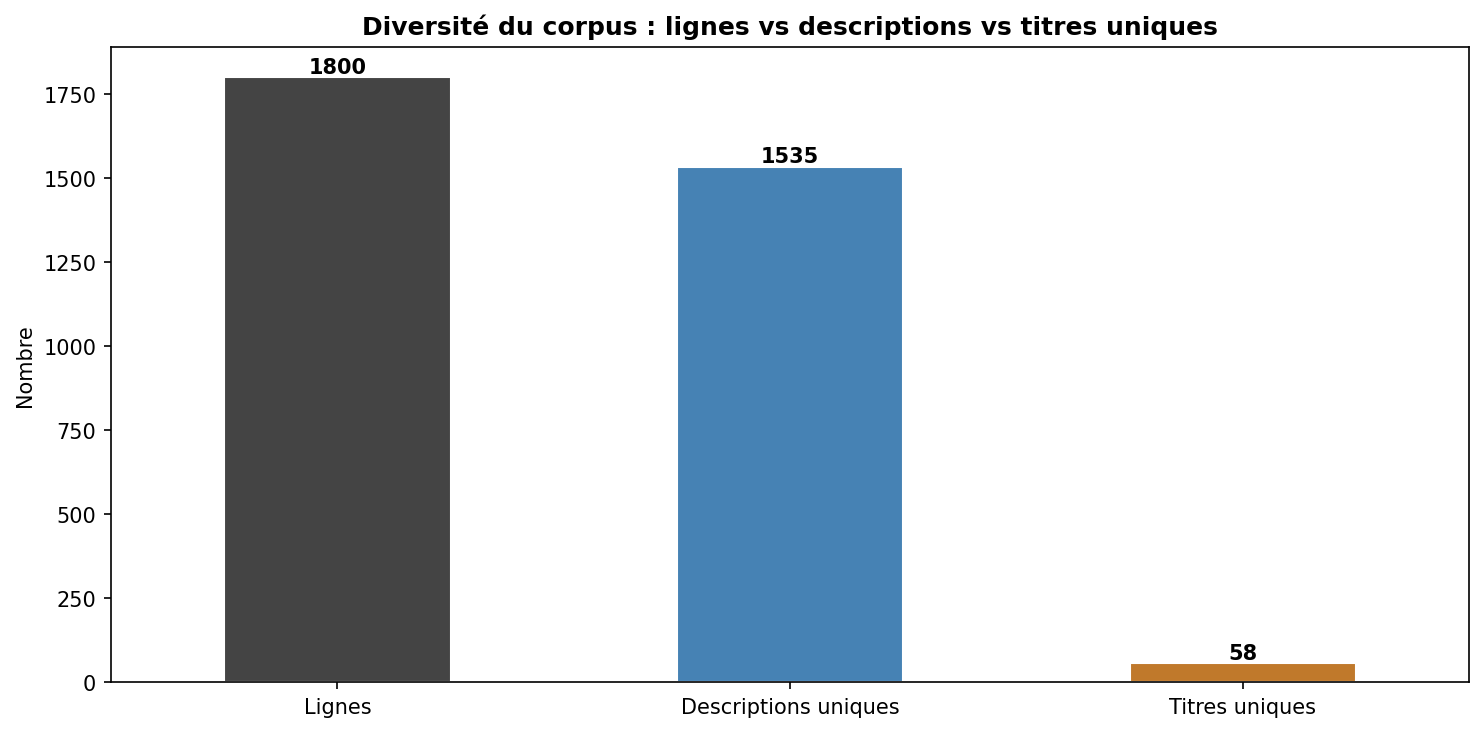
\includegraphics[width=0.90\textwidth]{ch03_redondance.png}
\caption{Diversité du corpus : lignes, descriptions et titres distincts}
\label{fig:redondance}
\end{figure}

La figure~\ref{fig:redondance} les rapproche. Pour 1\,800 lignes, nous dénombrons
1\,535 descriptions distinctes, soit 85\,\%. Les titres ne prennent que 58 valeurs distinctes, et le
champ \texttt{knowledge Base} en prend exactement autant. Le corpus s'organise donc autour de
58 types de tickets récurrents, chacun instancié en moyenne 31 fois avec des variations de surface :
demandeur, dates, identifiants de configuration, tournures de phrase.

La conséquence porte sur le protocole expérimental. Un découpage aléatoire placerait le même type de
ticket des deux côtés ; le modèle retrouverait au test un scénario déjà vu, et le score mesuré
refléterait sa capacité à mémoriser plutôt qu'à généraliser.

\section{Diagnostic de qualité et risques}

Les quatre analyses qui précèdent portent chacune sur un aspect du corpus. Cette section les
rassemble en un diagnostic unique, puis nomme les risques que ce diagnostic fait peser sur la suite
du travail et le traitement retenu pour chacun.

\subsection{Synthèse du diagnostic}

Les indicateurs du tableau~\ref{tab:dq} proviennent tous du script de diagnostic exécuté sur le
corpus, qui écrit ses résultats dans un fichier de métriques et engendre les figures de cette
section. Aucune valeur n'a été saisie à la main, ce qui rend le diagnostic reproductible à
l'identique.

\begin{table}[!htbp]
\centering
\styletableau
\caption{Synthèse du diagnostic de qualité}
\label{tab:dq}
\begin{tabular}{|Bp{5.0cm}|Lp{3.6cm}|Lp{4.2cm}|}
\hline
\rowcolor{enteteTab}
\textbf{Indicateur} & \textbf{Valeur} & \textbf{Lecture} \\
\hline
Lignes et champs & 1\,800 sur 18 champs & Volume exploitable \\
\hline
Catégories & 8 & Classification multi-classes \\
\hline
Déséquilibre maximal & 5,93 & À traiter en modélisation \\
\hline
Tickets vides & 0 & Aucun \\
\hline
Doublons de ligne complète & 0 & Aucun \\
\hline
Incohérences d'étiquetage & 0 & Annotation fiable \\
\hline
Descriptions distinctes & 1\,535 sur 1\,800 & Diversité satisfaisante \\
\hline
Titres distincts & 58 & Corpus organisé par scénarios \\
\hline
Longueur des descriptions & médiane 33 mots & Textes homogènes \\
\hline
Champs critiques manquants & 0 & Complétude assurée \\
\hline
\end{tabular}
\end{table}

Le corpus est structurellement sain. Ses difficultés portent sur la forme de sa distribution et sur
sa composition ; son intégrité est acquise.

\subsection{Risques identifiés et traitements retenus}

Le diagnostic qui précède fait apparaître des risques pour l'apprentissage. Le
tableau~\ref{tab:risques} associe à chacun son effet attendu sur les modèles et le traitement
décidé.

\begin{table}[!htbp]
\centering
\styletableau
\caption{Risques liés aux données et traitements associés}
\label{tab:risques}
\begin{tabular}{|Bp{3.2cm}|Lp{4.4cm}|Lp{5.2cm}|}
\hline
\rowcolor{enteteTab}
\textbf{Risque} & \textbf{Effet attendu} & \textbf{Traitement} \\
\hline
Déséquilibre des catégories & Rappel faible sur \emph{Sécurité} et \emph{Backup} & Métrique
F1-macro, pondération des classes, suivi du rappel par classe (chapitre~4) \\
\hline
Redondance des types de tickets & Fuite entre entraînement et test, scores surestimés & Découpage
par groupe de titres (section~\ref{sec:antifuite}) \\
\hline
Nettoyage trop agressif & Perte de signal lexical, généralisation dégradée & Révision des règles,
conservation du vocabulaire informatique \\
\hline
Champs incomplets & Base de connaissances lacunaire & Repli de \texttt{Résolution/Motif} sur
\texttt{knowledge Base} (chapitre~5) \\
\hline
Données personnelles en clair & Exposition de noms et de rattachements & Pseudonymisation par
empreinte à clé (chapitre~6) \\
\hline
\end{tabular}
\end{table}

\section{Limites du corpus}

\label{sec:representativite}

La section précédente traitait de risques que nous avons pu corriger. Celle-ci énonce une
limite que nous n'avons pas les moyens de lever : le corpus décrit fidèlement l'activité du service
support d'\OTBS sur quatorze mois, et rien de plus.

Sa composition en 58 scénarios récurrents en délimite la portée. Un modèle entraîné sur ces données
apprend à reconnaître des familles de problèmes déjà rencontrées ; le corpus ne permet pas de
mesurer sa capacité à traiter un problème inédit, faute d'y trouver de tels cas. Les performances
du chapitre~6 doivent se lire à cette échelle.

Deux restrictions de périmètre s'y ajoutent. Le corpus couvre les huit filiales du groupe et leur
parc applicatif, si bien que les résultats ne se transposent pas à une organisation dont le paysage
informatique diffère. Le référentiel de huit catégories est propre au service : un autre découpage
métier produirait un autre problème de classification.


% Aucun flottant du corps ne doit franchir la conclusion.
\FloatBarrier

\section*{Conclusion}
\addcontentsline{toc}{section}{Conclusion}

Le corpus est maintenant connu. Il compte 1\,800 tickets créés sur quatorze mois, décrits par
dix-huit champs dont quatre portent l'information exploitable. Sa distribution est inégale, la
catégorie la plus fréquente dépassant la plus rare d'un facteur 5,93.

Le constat déterminant est ailleurs. Pour 1\,800 lignes, le corpus ne porte que cinquante-huit
titres distincts, contre 1\,535 descriptions différentes. Le chapitre~1 lisait cet écart comme le
symptôme d'un travail répétitif ; mesuré ici, il devient une contrainte expérimentale, car tout
découpage qui ignore les titres mesurerait la mémorisation plutôt que la généralisation.

Les risques que ce diagnostic fait peser sont énoncés avec le traitement retenu pour chacun. Le
chapitre suivant ouvre la troisième phase et met ces traitements en œuvre.
